\newcommand{\bit}[1]{\textit{\textbf{#1}}}

\section{The workflow}
The workflow is divided into five major parts:
\begin{enumerate}
    \item Segmentation
    \item Electrode modeling \& positioning
    \item Volume mesh creation
    \item Simulation case setup and execution
    \item visualization and optionally
    \item \it{conductivity tensor estimation (optional)}.
\end{enumerate}
In this chapter, we describe the basic workflow for each of the mentioned stages of the workflow. For every stage of
the workflow, we describe the expected input and which output will be generated in a tabular format. You can replace
individual stages with your own workflow given that your workflow can handle the same input data and will create the
same output data. The order in which we describe the individual stages is the recommended processing order.

\subsection{Segmentation}
\begin{tabular}{ | p{0.2\textwidth} || p{0.75\textwidth} | }
    \hline
    \textbf{Input}  & Individual head MR image, T1-weighted (NIfTI file).\\
    \hline
    \textbf{Output} & Labeled image with one distinct label per structure (ANALYZE file) \\ 
    \hline
    \textbf{Tasks} & In this step of the workflow, an individual head MR images is segmented and based on
                     this segmentation, a labeled image is created. \\
    \hline
\end{tabular}

\hspace{0.5cm}

We have published an extended description of the segmentation workflow together with a user guide
\footnote{https://figshare.com/s/f2e47b41e974ab67039b} before \cite{kalloch2018semi}.\\
In the mentioned paper we describe the creation of surface-based head and torso models from individual 
MR images. For our tES workflow, only a sub-component of the described workflow namely the segmentation
of the head MR image is required. We perform the segmentation of the MR image of a
subject's head  in the same manner as described in that paper. We are able to segment skin, skull
and enclosed air cavities, cerebrospinal-fluid, gray matter, and white matter. Likewise, the segmentation
images are post-processed in the same manner. Finally, the result of this segmentation workflow that
we use further in our simulation workflow is a labeled image that contains the desired structures.\par
Note that other than described in the mentioned paper the topology of the segmented structure does not 
necessarily need to adhere a strictly nested arrangement. With our image-based meshing approach we
can create the volume mesh of structures of arbitrary arrangement, i.e. structures may intersect each
other or have common interfaces. This property is especially important when adding pathological
structures such as brain lesions after a stroke.


\subsection{Electrode Modeling}\label{sec:electrodemodeling}
\begin{tabular}{ | p{0.2\textwidth} || p{0.75\textwidth} | }
    \hline
    \textbf{Input}  & Iso-surface of the skin segmentation (STL file).\\
    \hline
    \textbf{Output} & Surface description of the electrode, (OFF file) \\ 
    \hline
    \textbf{Tasks} & In this step of the workflow, the electrodes modeled (shape \& location on scalp).
                     A surface description of the final electrodes is created.\\
    \hline
\end{tabular}

\hspace{0.5cm}

The electrode modeling and positioning is implemented as a plugin for the 3D modeling software Blender.
To install the plugin in blender copy \& paste the file \emph{mountElectrode.py} into the plugin folder
of your Blender installation. In Ubuntu this folder is usually located in the ``.config" directory
of your home directory:
\newline
\colorbox{lightgray}{\$HOME/.config/blender/2.79/scripts/addons/}.
\newline
In Blender enable the plugin via: File $\Rightarrow$ User Preferences $\Rightarrow$ Search in the list
of plugins for "Object: Mount Electrodes" $\Rightarrow$ tick it.
\par
After successful installation you will be presented with the following user interface.
\begin{figure}[H]
   \centering
   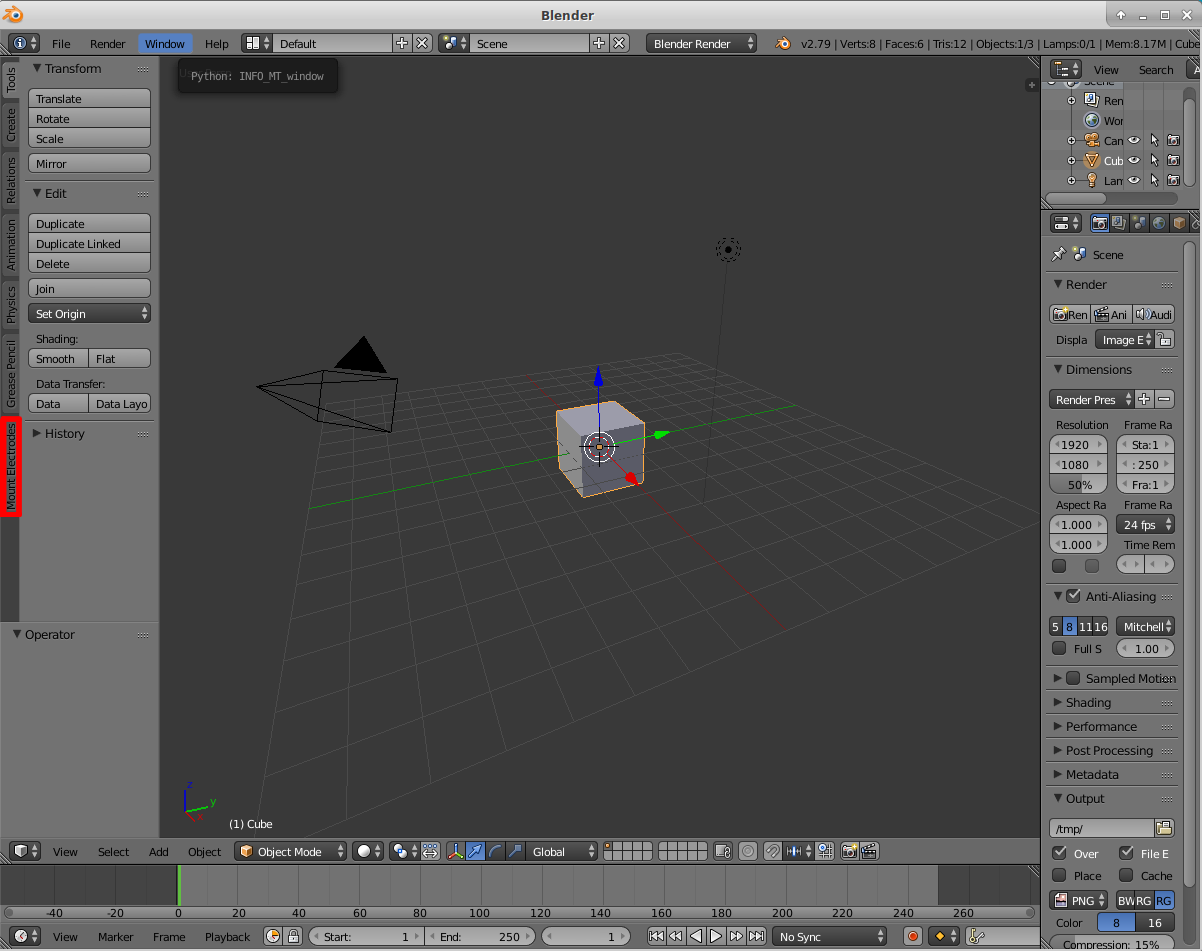
\includegraphics[width=1\textwidth]{blender_1}
   \caption{\emph{Standard Blender UI after enabling the Mount Electrodes plugin.}}
\end{figure}
You can activate the UI of the plugin by clicking the ``Mount Electrodes" tab on the left pane.
\begin{figure}[H]
   \centering
   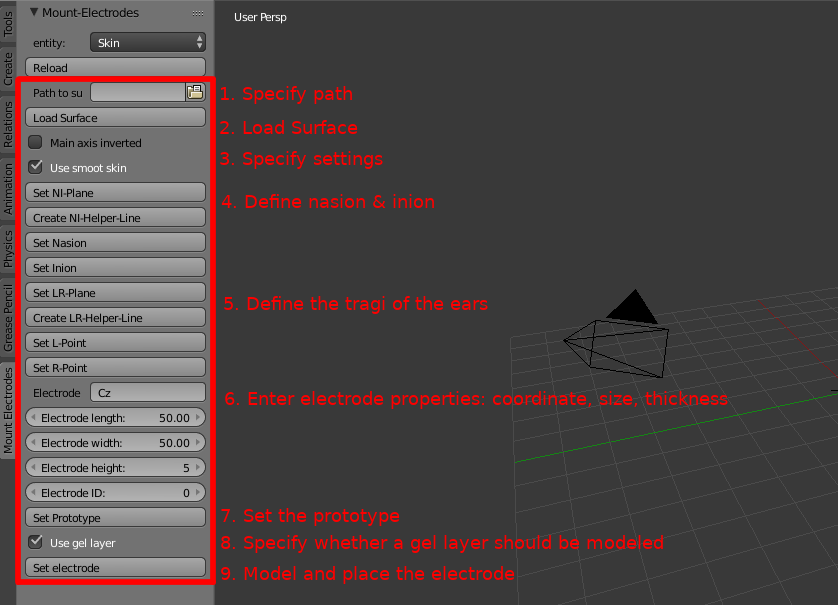
\includegraphics[width=1\textwidth]{blender_2}
   \caption{\emph{UI of the Mount Electrodes plugin.}}
\end{figure}
First, you need to specify the path to an STL surface file that describes the surface of the skin
of the model you want to mount the electrodes to. This surface must be generated in external software,
for example, in ParaView using the ``Contour filter" in ParaView from the binarized version of the
labeled image file that used during volume meshing later. Then click `Load Surface".
This step may take a couple of minutes as the plugin computes a smoothed version of the input surface
simultaneously.\par
The checkbox ``main axis" inverted defines whether the head surface faces the down or up the z-axis.
If your subject is oriented in the standard axial orientation, it is not required to check this.\par
\begin{figure}[H]
   \centering
   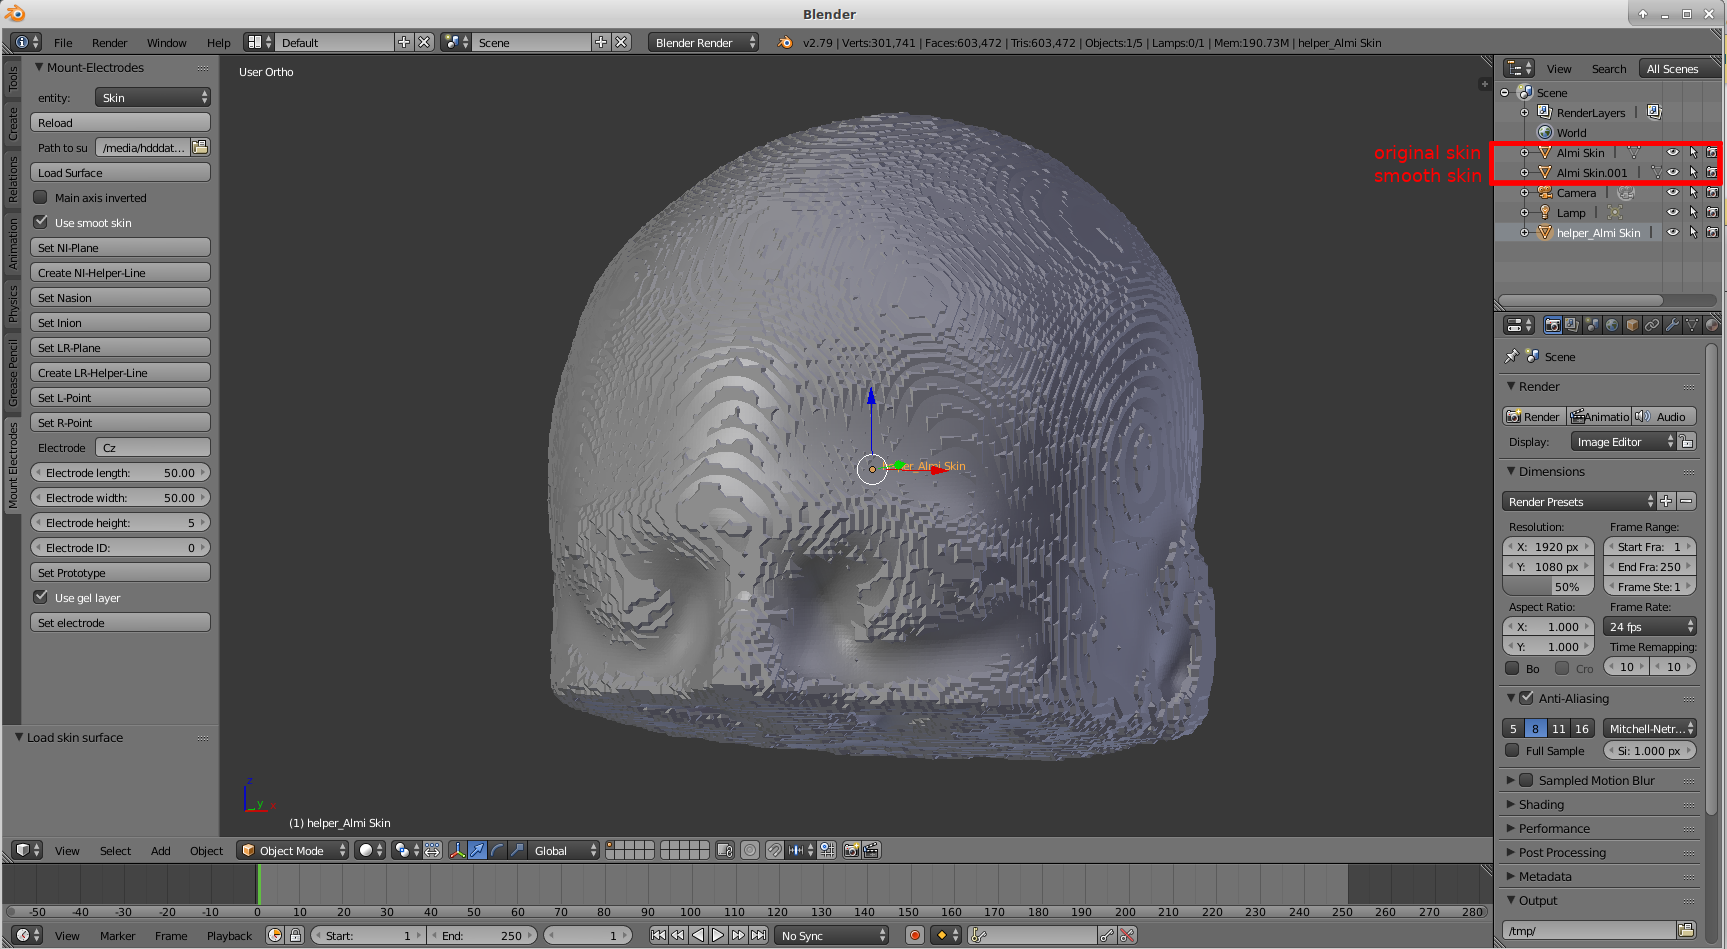
\includegraphics[width=1\textwidth]{blender_3}
   \caption{\emph{Loaded skin surface. Notice how both, the original version as created by the
                  Marching Cubes algorithm as well as a smooth version (mainly covered by the
                  original version) are shown.}}
\end{figure}
The option ``use smooth skin" defines whether the original skin surface or the smoothed version
of the skin surface should be used for the electrode modeling. You should use the original surface
if you are attempting a full image-based meshing of the head. Otherwise, to perform a surface-based
meshing of the skin and an image-based meshing of all other tissues use the smoothed version to
benefit from the greater smoothness and thereby more accurate modeling of the edges of the electrode.
Note that the electrodes will always be meshed by a surface-based approach regardless of the skin
will be meshed by an image-based or surface-based approach.\par
Your next task is to align the nasion-inion plane to the center of the head. The center position
is precomputed by the plugin, but a correction might be necessary. You can manipulate the location
using the red arrow in the center of the plane. If the head is tilted a rotation of the plane might
be necessary. To perform a rotation, use the ``R" button on the keyboard followed by the letter of
the axis around which the plane should be rotated. Once you are satisfied with the alignment of the
NI-plane click ``Create NI-Helper-Line". On the created line, click with the right mouse button
at the location of the nasion, the chosen point will be highlighted at the ni-line, then click 
``Set Nasion". The plugin computes the location of the nasion automatically, but a correction might
be necessary. Next, right-click at the location of the inion, then click ``Set Inion". You should
notice that the length of the NI-line was reduced.
\begin{figure}[H]
   \centering
   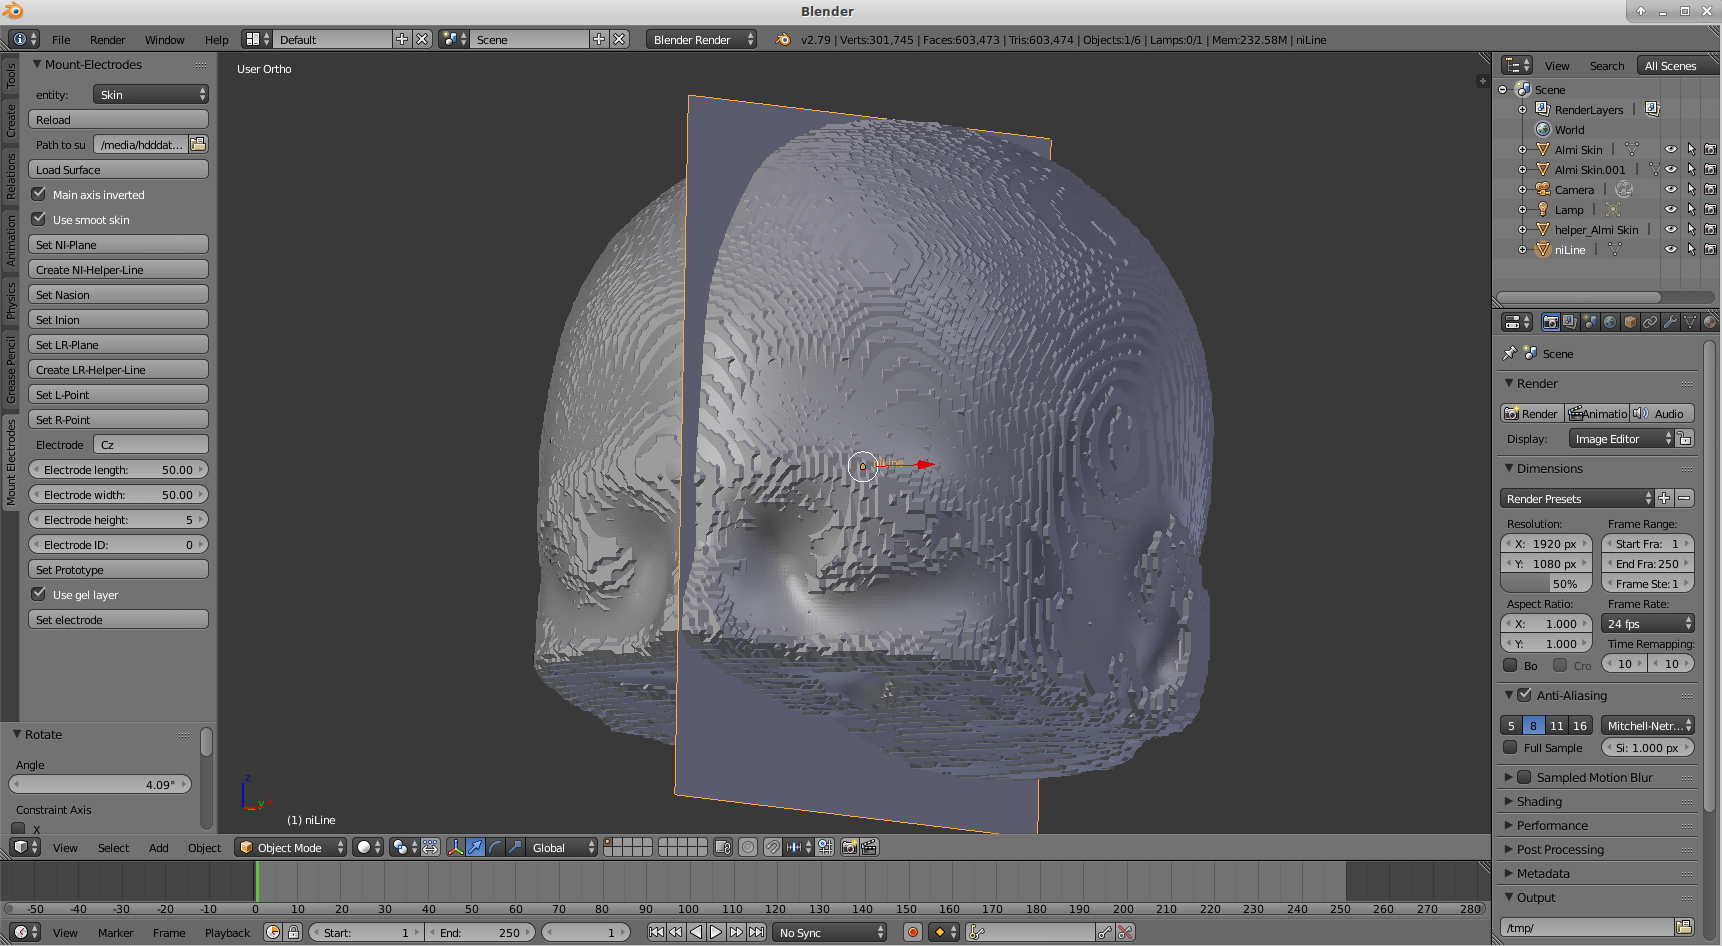
\includegraphics[width=1\textwidth]{blender_4}
   \caption{\emph{NI-plane set.a}}
\end{figure}
\begin{figure}[H]
   \centering
   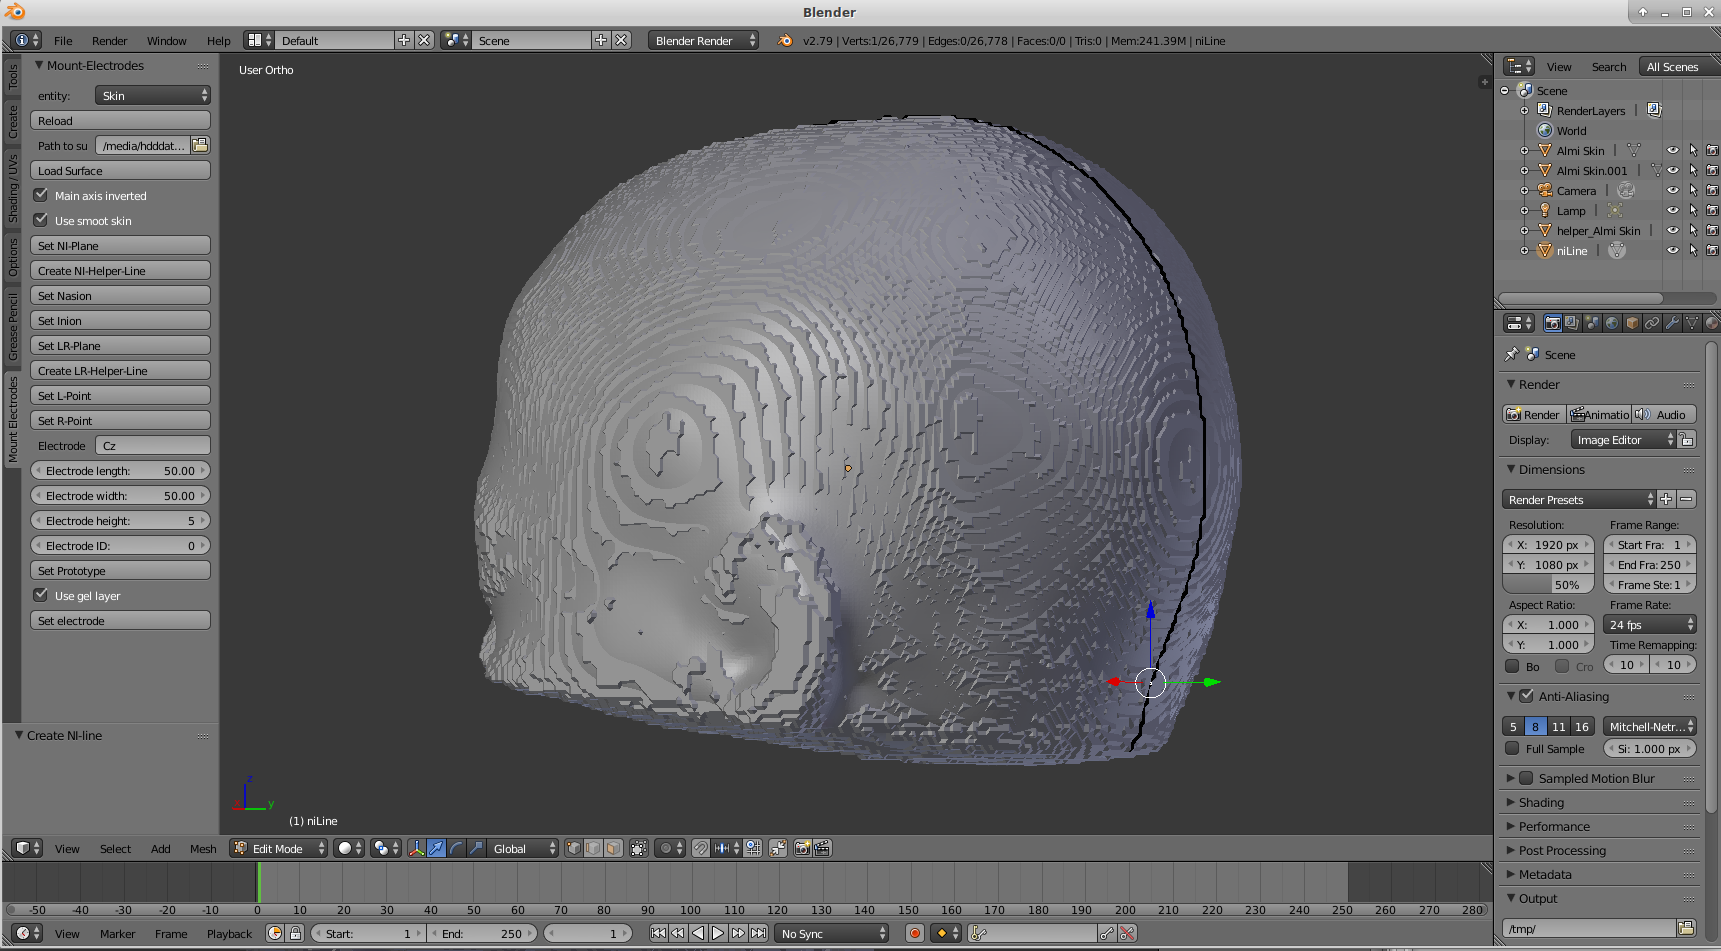
\includegraphics[width=1\textwidth]{blender_5}
   \caption{\emph{Inion defined-plane set.}}
\end{figure}
Perform the definition of the tragi of the ears in a similar fashion: first, align the helper plane,
create the lr-line and define the point on the right and on the left.
\begin{figure}[H]
   \centering
   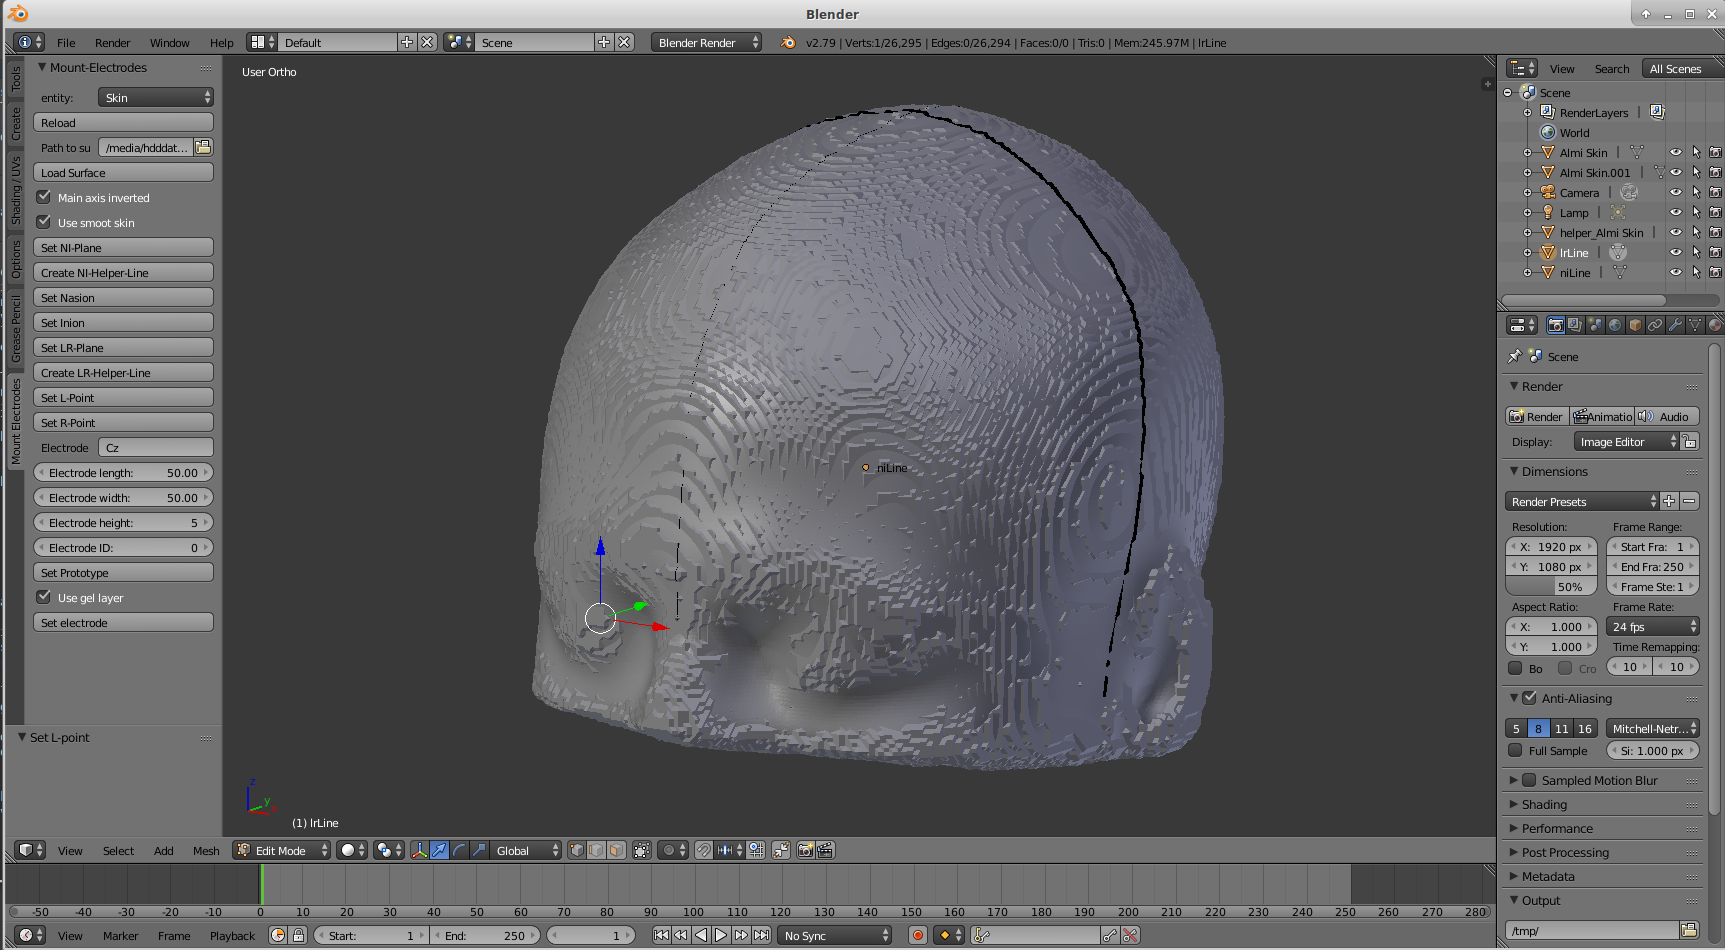
\includegraphics[width=1\textwidth]{blender_6}
   \caption{\emph{LR-line defined.}}
\end{figure}
Next, the properties of the electrodes must be entered. First, enter the position according to the
international 10-12 system. Then define the shape parameters of the electrodes. You do not need to
modify the electrode-id as this will be auto-incremented with every new electrode you place.\par
After defining the electrode parameters click ``Set Prototype". A cube of the specified size will
appear the specified location. You can adjust the position of the cube manually if the placement is
unsatisfactory. You could even change the shape of the cube by modifying its geometry. This is how
we modeled the triangular electrode.
\begin{figure}[H]
   \centering
   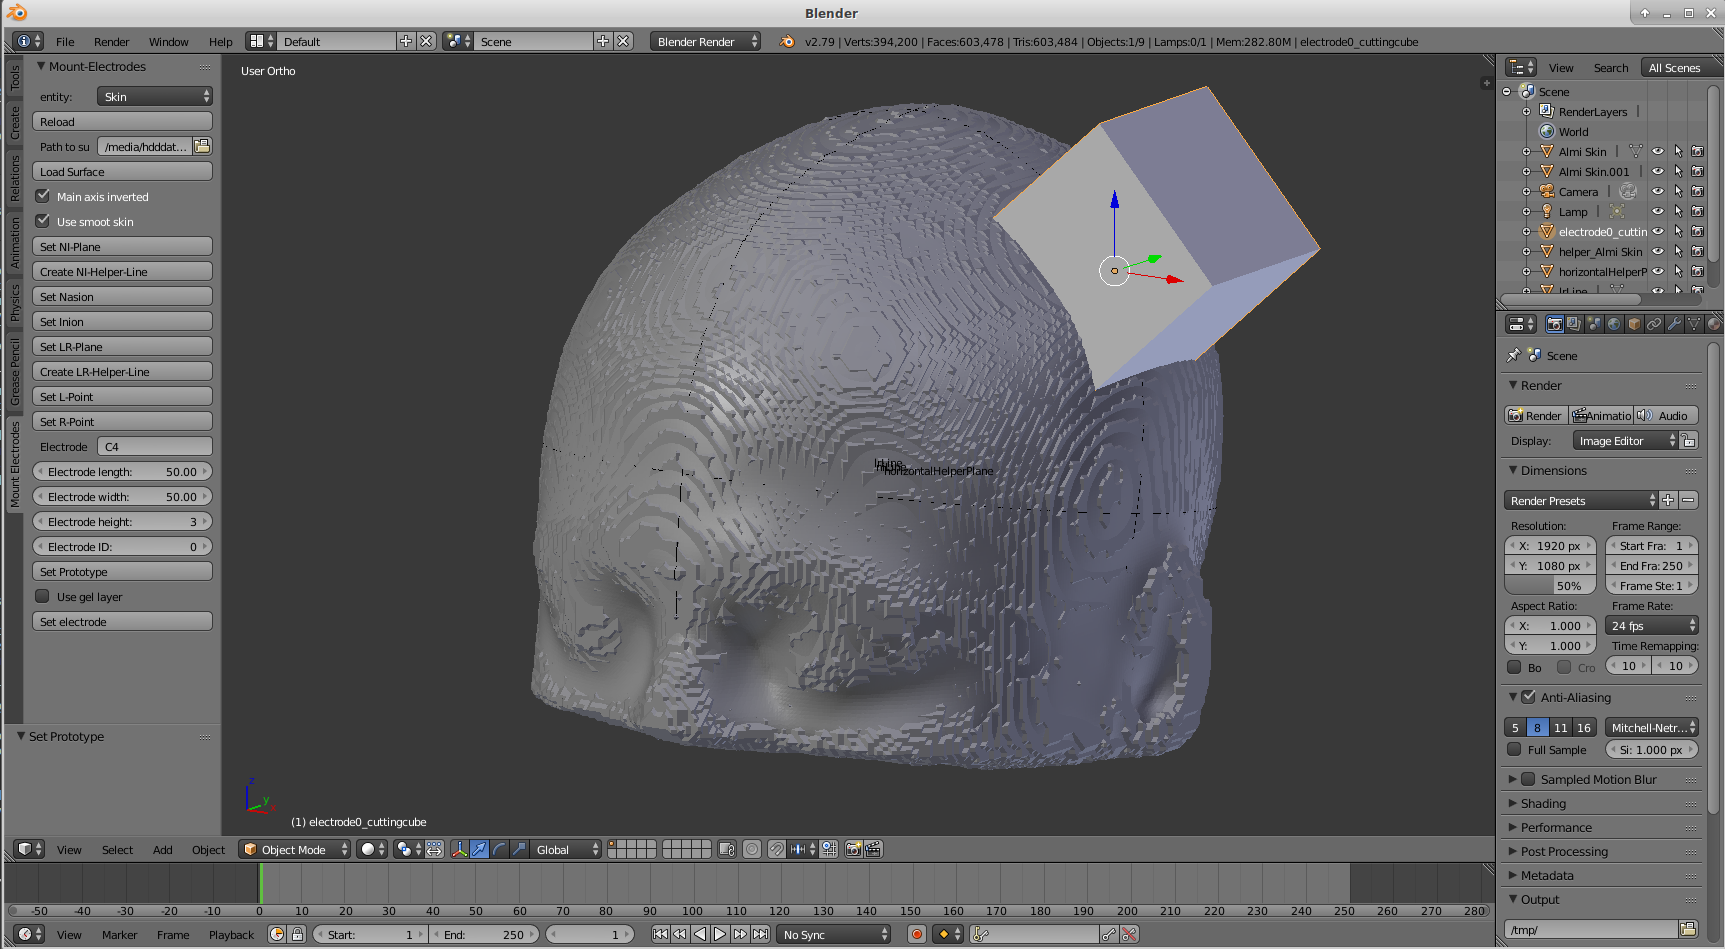
\includegraphics[width=1\textwidth]{blender_7}
   \caption{\emph{Prototype set at C4.}}
\end{figure}
You may finally decide to use a gel layer underneath the electrode and the model and place the 
electrode by clicking ``Set electrode". The electrode will be placed at the location of the cube,
with the same extents and the specified thickness.
\begin{figure}[H]
   \centering
   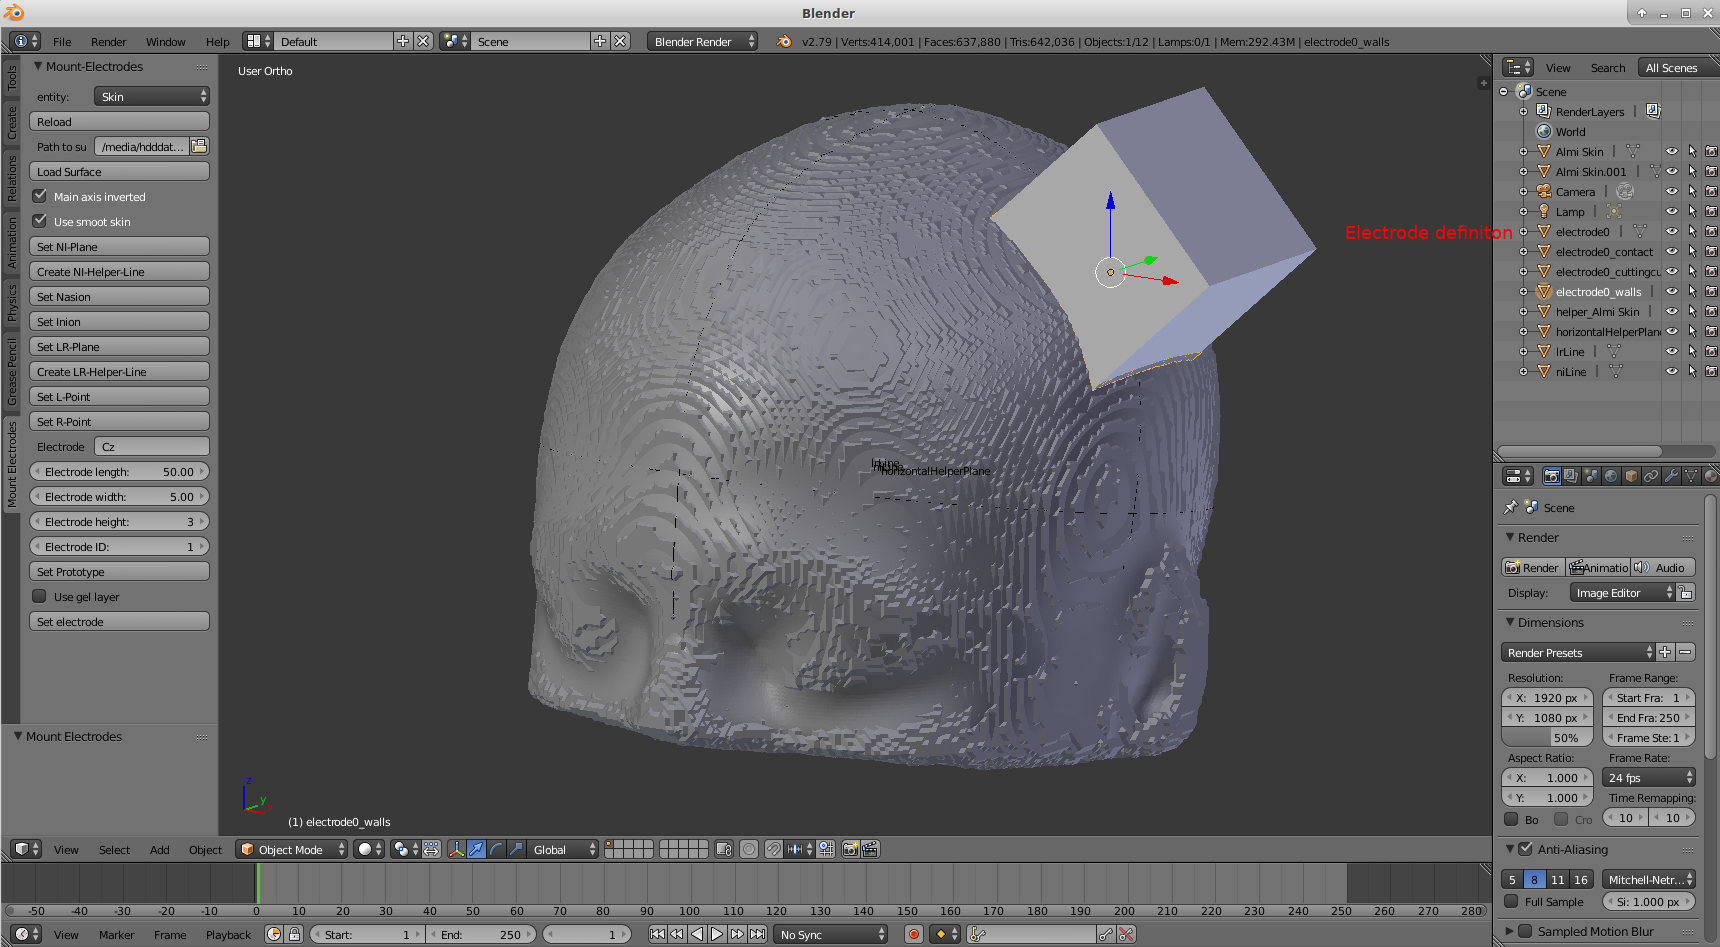
\includegraphics[width=1\textwidth]{blender_8}
   \caption{\emph{Electrode modeled and ready for export.}}
\end{figure}
You can export the electrode by left clicking the name ``electrodeX" (where X = id of the electrode)
and then \emph{File} $\Rightarrow$ \emph{Export} $\Rightarrow$ \emph{STL}. Make sure to check the
option ``Selection Only" and then specify the file name and path where to save the electrode.\par
To use the surface description of the electrode in our meshing tool we must convert it into the
Object File Format (OFF). We do this in Meshlab. Import the STL file of the electrodes. When importing
Meshlab prompts to unify duplicate vertices. Do this. Next, reduce the number of triangles and clean
the surface description. If you modeled the electrodes according to the original surface, i.e. the electrode
doe not have a smooth surface, but this typical jagged surface due to the Marching Cubes algorithm
then use the filter \emph{Filter} $\Rightarrow$ \emph{Remeshing, Simplification, Reconstruction}
$\Rightarrow$ \emph{Simplification: MC edge collapse}. Else, i.e. you modeled the electrode using the
smooth skin surface and therefore also have a smooth electrode, use the filter \emph{Filter} $\Rightarrow$
\emph{Remeshing, Simplification, Reconstruction} $\Rightarrow$ \emph{Quadaratic Edge Collapse Decimation}
and specify the parameters as ``Quality = 1", tick ``Preserve Boundary of the mesh", and tick ``Planar 
simplification". Finally ``Export Mesh as" an OFF file under the File menu.

\subsection{Volume Mesh Generation}
\begin{tabular}{ | p{0.2\textwidth} || p{0.75\textwidth} | }
    \hline
    \textbf{Input}  & \emph{Option 1)} Labeled image containing all segmented head structure (ANALYZE file) + 
                      electrode definitions (OFF file) \newline
                      \emph{Option 2)} Labeled image containing all segmented head structures but the skin
                      structure (ANALYZE file) +  smooth surface representation of the skin (OFF file)
                      + electrode definitions (OFF file) 
                      \emph{Option 3)} Labeled image containing some irregular structures (e.g. lesioned tissue) (ANALYZE file) + 
                      surface representation of other tissue structures (e.g. skin, skull, CSF, GM, WM) (OFF file) +
                      electrode definitions (OFF file)\\
    \hline
    \textbf{Output} & Tetrahedral volume mesh of the head with the electrodes mounted, boundaries of the
                      electrodes represented as ``Physical Surfaces" (GMSH file format v2). \\
    \hline
    \textbf{Tasks} & In this step of the workflow a tetrahedral volume mesh is generated using a combination
                     of an image-based as well as surface-based meshing approach.\\
    \hline
\end{tabular}

\hspace{0.5cm}

The volume mesh generation is implemented as a C++ tool using the API of CGAL v. 4.13.1 and GMSH v. 4.3.
Follow the instructions of the README file of the MeshHeadModel submodule to compile the application.
For convenience, we provide a Docker file that creates a Docker container based on Ubuntu 19.04
that contains all required dependencies. You can then compile and execute the application within the container
using the two provided scripts. All that is left to do in that case is to adapt the paths and container name
in the scripts to your configuration and to download, extract and compile the GMSH source code.\par
The mode of standard operation is an image-based meshing meaning that in any case, you must at least provide a
labeled image file in the ANALYZE file format as an input and the name of the output mesh. All other arguments
are optional.\par
The image-based meshing operation will create a tetrahedral volume mesh with one separate mesh compartment
(in GMSH terminology: 'Physical Volume') per label found in the input image. Since the boundaries of these
compartments are determined dynamically via bisection during the meshing process, the labels within the 
input images do not need to adhere any special constraints in terms of the topology of the represented 
structure. The individual mesh compartments are named in a numerically increasing order representing the
order of their corresponding labels in the input image file. For compatibility with OpenFOAM, the boundary
of the generated mesh compartments are not explicitly saved when exporting the mesh to the GMSH file
format meaning that no separate boundary surface (in GMSH terminology: 'Physical Surface') of the structures
in the input image will be generated. The reason for this is when converting the GMSH mesh into the OpenFOAM file
format any preserved boundaries will be converted to an OpenFOAM 'patch' at which boundary conditions may be
defined. However, by definition mesh boundaries or 'patches' must only be defined at the outer boundary of
the mesh. A definition of an internal 'patch' is invalid and will raise a warning during conversion.\par
To include electrodes into the model you must specify the path to their surface descriptions in Object File 
Format (OFF) via the parameter 'electrodefiles'. This surface will be meshed using a feature-preserving 
surface-based meshing approach. Therefore, they must be of good quality as discussed at the end of section
\ref{sec:electrodemodeling}. Features edges with an inner angle smaller than 60 degrees will be preserved.
The electrodes will be represented both as individual mesh compartments, i.e. 'Physical Volumes', and by
their boundaries, i.e. 'Physical Surfaces'. Preserving an explicit description of their boundary is required
to define the boundary conditions of the simulation later in OpenFOAM. The volume compartments of the mesh
representing the electrodes will always be the last 'n' compartments (with n = \#electrodes). Together with
the input image the order of mesh compartments is then: image-based structures $\Rightarrow$ electrodes.\par
The boundary of the meshed structures generated by the image-based meshing algorithm may not be as smooth as
a smoothed surface-based meshed. This is especially disadvantageous in the case of the electrode representations
and their contact surface with the scalp. Therefore, you may provide a smooth surface file of the skin and the
corresponding smooth electrodes. You must specify the path to the smooth skin surface description with the parameter
'tissuesurfaces', again as an OFF file. The quality of this surface file must be adequate. Note that in
this case, the order of mesh compartments is as follows: image-based structures $\Rightarrow$ smooth
skin $\Rightarrow$ electrodes. Again, the boundary surface of the skin compartment is not exported to the
GMSH file format to avoid incompatibilities in OpenFOAM.\par
Finally, if your application requires a more precise approximation of the boundaries of the structures than
it is achieved using the image-based meshing approach you may provide the surface definitions of additional
internal structures (as OFF files) which will then be meshed using the surface-based meshing approach. Note
that these surfaces must be of very good quality. To achieve adequate surfaces, we recommend the application
of the \emph{Taubin smoothing} functionality of MeshLab to first, smooth the surface, then the tool \emph{MeshFix}
by Marco Attene \cite{attene2010lightweight} to ensure an appropriate mesh quality and finally our
\emph{surface-remesh tool}. The order of the provided surfaces
must begin with the most outer structure (i.e. usually this will be the skin surface) and it must end with
the most inner structure (e.g. the gray matter structure). Additional inner structures may still be represented
using a labeled image, for example, to represent lesioned tissue or the ventricles. A typical use case is to
create the volume mesh based on surfaces for the typical structures (electrodes, skin, skull, cerebrospinal
fluid, gray matter, white matter) and add irregular tissue such as lesioned tissue by providing a corresponding
labeled image. It is completely unproblematic if the structures in the image intersect the provided surfaces
in the final volume mesh. The intersection will also be visible in the final mesh. In the final volume mesh,
the order of mesh compartments is as follows: image-based structures $\Rightarrow$ skin $\Rightarrow$ skull
$\Rightarrow$ csf $\Rightarrow$ gm $\Rightarrow$ wm $\Rightarrow$ electrodes. Again, only the boundary surfaces
of the electrodes is exported to the GMSH file format to avoid incompatibilities in OpenFOAM.\par

\begin{figure}[H]
   \centering
   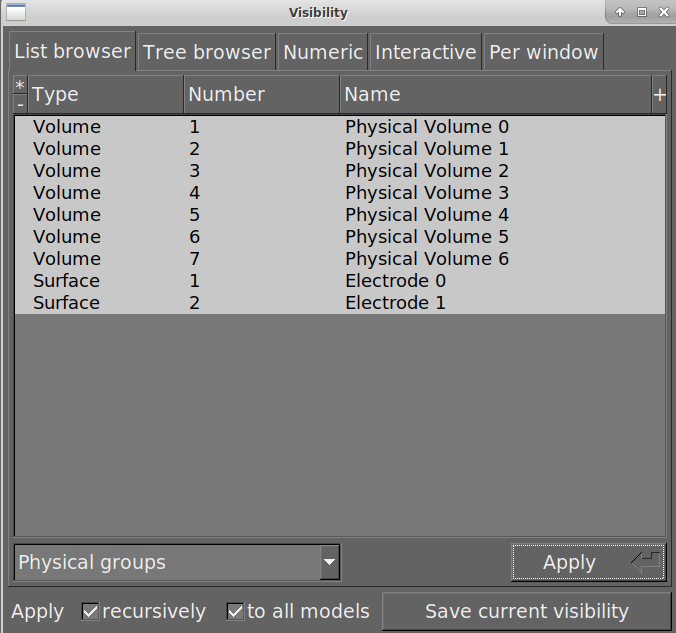
\includegraphics[width=0.5\textwidth]{gmsh}
   \caption{\emph{Mesh compartments and boundaries of the almi5 test mesh using a smooth skin
    representation. Physical Volume 0 = skull,
    Physical Volume 1 = CSF, Physical Volume 2 = GM, Physical Volume 3 = WM, Physical Volume 4 = skin,
    Physical Volume 5 = volume of electrode 0, Physical Volume 6 = volume electrode 1, Electrode 0 =
    boundary definition of electrode 0, Electrode 1 = boundary definition of electrode 1.}}
\end{figure}
Additional parameters concern the mesh element size and quality (\url{https://doc.cgal.org/4.12/Mesh_3/index.html#title11})
and the mesh optimization phases (\url{https://doc.cgal.org/4.12/Mesh_3/index.html#title6}). Please refer
to the provided online resources of the CGAL library for their explanation. The configuration of 
parameters that we typically use is predefined in the script file 'runMeshingTool.sh'.

\subsection{Simulation Case Setup}
\begin{tabular}{ | p{0.2\textwidth} || p{0.75\textwidth} | }
    \hline
    \textbf{Input}  & Tetrahedral volume mesh of the head. (GMSH file format v2) \\
    \hline
    \textbf{Output} & Electrical field strength (E), Electrical Current Density (J), Magnitude of
                      E and J. (OpenFOAM file format) \\ 
    \hline
    \textbf{Tasks} & In this step of the workflow we perform the electric field calculations. \\
    \hline
\end{tabular}

\hspace{0.5cm}

We use OpenFOAM as a software suite to perform our simulations. Therefore, you first must make sure
to set OpenFOAM up properly and compile our TDCSSolver accordingly.\par
OpenFOAM provides a set of command line tools to set up and execute a test case. Therefore a strict
structure of the simulation directory must be maintained:
\begin{itemize}
    \item \textbf{0} - The 0 directory contains the boundary conditions and initial values for all fields.
                       Each field is represented by one file containing a so-called dictionary the defines
                       the internal field values and the boundary conditions.\par
                       The solver application will create more directories with numeric names representing
                       the iteration in which the solution converged. The directory with the highest number
                       contains the result.
    \item \textbf{constant} - The constant directory contains all static properties of the test case. In our
                              case of tES simulation, this is only the mesh.
    \item \textbf{system} - The system directory contains all configuration files to control the setup and
                            execution of the test case. These include: a) \emph{controlDict} (information about the
                            employed solver application, runtime behavior, maximum number of outer iterations,
                            as well as precision, format and frequency of writing results), b) \emph{fvSchemes}
                            (numerical discretization schemes of the involved operators, in our case for the divergence-,
                            gradient- and Laplace-operator), c) \emph{fvSolution} (control of the equation solver,
                            solver tolerance, maximum/minimum number of iterations, relaxation factors, number
                            of non-orthogonal corrector iterations), d) \emph{setFieldsDict} (initial field values
                            for all mesh compartments, in our case the initial conductivity values), e)
                            \emph{solverProperties} (parameters for our TDCSSolver, number of electrodes, name of
                            the contact surface of the electrodes (always 'faceZone\_n' with 
                            n=[0...(\#electrodes - 1)]) and the desired input current strength. 
\end{itemize}
Please refer to the 'test\_case\_stubs' of the 'utils' submodule for an exemplary test case folder setup. Note
that this basic structure can be copied to any new test case. To prepare a test case folder for a new test case
the following steps must be executed:
\begin{enumerate}
    \item \textbf{Import the mesh}: Using the tool \emph{gmshToFoam} you can import the GMSH volume mesh files
    created by our meshing tool. After successful import, downscale the mesh accordingly since 1 unit of measurement
    corresponds to 1m in OpenFOAM. Therefore, a mesh generated from an MRI of 1 mm isotropic resolution must be
    downscaled by 0.001: \emph{transformPoints -scale '(0.001 0.001 0.001)'}.

    \item \textbf{Set boundary conditions}: Create the 0 directory with files for both the conductivity (\emph{sigma})
    and the electrical potential (\emph{ElPot}). In bohth cases, the \emph{boundaryField} dictionary must contain
    sub-dictionaries for each electrode (denoted by 'patchn' with n=[0...(1 - \#electrodes)]). We apply a Dirichlet
    boundary condition in both cases. The 'defaultFaces' boundary must be present as well. This boundary represents
    all non-electrode outer boundaries of the mesh (i.e. the scalp that is not in contact with the electrodes).

    \item \textbf{Set initial values}: We set the initial field values using the \emph{setFields} tool. This
    tool reads the 'setFieldsDict' file. Therefore, you first must adapt that file according to your test case.
    You must specify the conductivity value for each mesh compartment in that file. Note that mesh compartments
    are defined by \emph{cellZones} in OpenFOAM. The order of the cellZones is the same as the order of the
    'Physical Volumes' in GMSH. This order can be verified in GMSH using the visibility menu.\\
    After you successfully adapted the \emph{setFieldsDict} file just run \emph{setFields}. The tool will populate
    the 'internalField' dictionary of \emph{sigma} for each cell of the mesh with the specified conductivity value 
    according to their membership to the mesh compartments.

    \item \textbf{Define application solver parameters}: You must specify the target input current strength, as well
    as the number of electrodes and the names of their contact surfaces. When importing the GMSH mesh into OpenFOAM
    the contact surfaces will be stored as \emph{faceZones}. Therefore, when importing the mesh from our meshing tool
    you must specify the names separated by a white space as 'faceZone\_n', again with n=[0...(1 - \#electrodes)]).

    \item \textbf{Run the simulation}: Depending on the quality of the input mesh you may have to adjust the
    convergence criteria in the \emph{fvSolution} file. You may decrease the relaxation factor for an under-
    relaxation of the system or further decrease the 'tolerance' parameter of the solver solving the E field.
    In severe cases of bad mesh quality, you may enable a limiter in the Laplace scheme to avoid over-shoots
    in the subsequent gradient calculations (laplacian(sigma,ElPot)  Gauss linear limited 0.5). Our meshing
    tool typically generates meshes of adequate quality. Therefore, it should not be necessary to use any of
    these means.\\
    You may run the simulation by executing the \emph{TDCSSolver}.

    \item \textbf{Visualize the result}: Run \emph{ParaFoam} to visualize the result. Please refer to
    \url{https://www.openfoam.com/documentation/user-guide/paraview.php} for an explanation for the ParaView
    user interface when visualizing an OpenFOAM test case.
\end{enumerate}

\subsection{Incorporating Diffusion-Weighted Imaging Data}
\begin{tabular}{ | p{0.2\textwidth} || p{0.75\textwidth} | }
    \hline
    \textbf{Input}  & DWI data of the subject, b-value, b-vector files. \\
    \hline
    \textbf{Output} & Conductivity tensors (OpenFOAM field file format) \\
    \hline
    \textbf{Tasks} & In this step we preprocess the DWI data of the subject, compute the
                     diffusion tensors, convert them to conductivity tensors and export them
                     in OpenFOAM field file format.\\
    \hline
\end{tabular}

\hspace{0.5cm}

The conductivity values of a simulation case can be enriched by information derived from DWI data of the subject.
In order to incorporate this information we suggest a workflow based on MRTtrix3 for data preprocessing and ParaView
for the computation of the conductivity tensors.\par
The recommended processing workflow in MRTrix3 is:
\begin{enumerate}
    \item \textbf{dwidenoise} - Perform denoising of the DWI data.
    \item \textbf{dwipreproc} - Motion \& eddy current correction.
    \item \textbf{dwi2mask} - Create a brain mask.
    \item \textbf{dwibiascorrect} - Correct magnetic field inhomogeneities (only in the brain using the computed mask).
    \item \textbf{dwi2tensor} - Compute diffusion tensors.
    \item \textbf{tensor2mestric} - Compute the fractional anisotropy map. 
    \item \textbf{fslmaths} - Remove NaN values from both the DTI image as well the FA map using 
          `fslmaths IMAGE\_FILE\_NAME -nan OUTIMAGE\_FILE\_NAME"
\end{enumerate}
The next step is to register the DTI data into the space of the T1-weighted ANALYZE image. It is important to use the same
ANALYZE image of the subject that was used for the mesh generation as well. This way the registered tensor data will
align well with the white matter compartment of the mesh. Using \emph{FSL Flirt}, we first perform an affine
registration of the FA map to the T1 image and save the computed transformation matrix. Since both images are of different
sequences we use the `mutualinfo" cost function for this registration. Second, we perform a non-linear registration of the
linearly registered FA map to the T1 image using \emph{FSL Fnirt}. Again we save the warpfield describing the transformation.
We then apply both the linear registration matrix and the non-linear warpfield to the DWI data using \emph{FSL vecreg}
and thereby ensure the preservation of the tensor orientation.\par
The subsequent conversion from diffusion tensors to conductivity tensors will be performed in ParaView. However, the
NIfTI reader module of ParaView may not load NIfTI files with multi-component values such as tensor data properly. Therefore,
we convert the NIfTI file to a vtkImage using \emph{ITKSnap}.\par
The generate VTK file can be opened in ParaView. In the simulation directory launch `paraFoam" since we need the mesh of the
simulation case as well. Then perform the following sequence of filters to the DTI data (filter marked with * are custom
filters that are provided as submodules of this repository):
\begin{enumerate}
    \item \textbf{Transform filter} - Scale down the image file to match the extents of the mesh. This typically involves
                                      a downscaling by 0.001.
    \item \textbf{SynMatixToGenMatrix filter [*]} - We inflate the 6-element symmetric tensor to a 9-element tensor as:
            \begin{equation}
                \begin{vmatrix}
                    a & d & f \\
                    \cdot & b & e \\
                    \cdot & \cdot & b
                \end{vmatrix}
                =
                \begin{vmatrix}
                    a & d & f \\
                    d & b & e \\
                    f & e & c
                \end{vmatrix}
            \end{equation}
    \item \textbf{DiffusionTensorToConductivityTensor filter [*]} - We convert the diffusion tensors to conductivity tensors
                                                                    according to volume-constraint method \cite{wolters2006influence}.
    \item \textbf{ResampleWithDataset filter} - We resample the diffusion tensors onto the `internal mesh" of the simulation
                                                case. Choose `Conductivity Tensors" as `Input" and `Head Mesh" as
                                                the `Source" in the filter options.
    \item \textbf{PointDataToCellData} - OpenFOAM reads and writes field values as cell data, i.e. one value that is valid
                                         within the entire cell. However, our image data are defined as point data, i.e. data
                                         that are defined on the vertices of the mesh. To successfully transfer the conductivity
                                         tensors to an OpenFOAM field we interpolate the data defined on the mesh points to
                                         the cells. Note that the filter must be executed on the resampled dataset.
    \item \textbf{SaveAsOFField [*]} - The last task will be to export the field data into an OpenFOAM conform field data format.
                                       Use this custom filter and specify a target path for the output file. Alternatively,
                                       you may export it as a CSV file in a list format.
\end{enumerate}
Finally, you may transfer the exported field data onto the \emph{sigma} field of the simulation case using the 
\emph{mapToFOAMField.py} Python script. Expected input parameters are a) a list file containing the values that should
be mapped, and b) the path to the OpenFOAM field file. Note that a) must not be an OpenFOAM field. Therefore, if you exported
the conductivity tensors using the SaveAsOFField filter you must remove the OpenFOAM header of the file and the closing
bracket at the end of the file and just retain the list of field values (one tensor-value per line).
